%
% $Id: blank.tex,v 2.0 2010-01-05 18:50:50+09 kobayasi Exp $
%
% Mar 21, 2001:  Revision Control Started!!
%
\documentclass[11pt]{jarticle}
\usepackage{newcent}             % PDFへの変換後の品質を高める
\usepackage[dvipdfmx]{graphicx}
\usepackage{wrapfig} % 文章を図に回り込ませて配置するもの
\usepackage{comment} % 複数行をコメントアウトするためのもの
\usepackage{color}
\definecolor{purple}{rgb}{0.6,0,0.4}
\definecolor{brown}{cmyk}{0,0.81,1,0.60}
\usepackage{listings, jlisting}
\renewcommand{\lstlistingname}{ソース}
\lstset
{
breaklines = true,
language=Java,
keywordstyle={\color{purple}},
commentstyle={\color{brown}},
numbers=left,
frame=single,
tabsize=4
}


%
%\usepackage[doctor]{gaiyo}      % 博士論文要旨の場合
%\usepackage[master]{gaiyo}      % 修士論文要旨の場合
\usepackage[senior]{gaiyo}               % 卒業研究概要の場合
% \usepackage[junior]{gaiyo}      % 専門演習レポートの場合

\title{スマートフォンのモーションセンサを利用した個人認証アプリケーションの開発}
\id{情11-170}
\author{高坂 賢佑}
\teacher{小林 孝史}

\begin{document}
\maketitle

\section{はじめに}
スマートフォンが徐々に普及しつつある現在,スマートフォンの個人認証方法は画面上に表示されるソフトウェアキーボードのテンキーを用いたパスコード認証が大部分を占めている.
しかし,この認証方法は画面ロックを解除するたびに画面に表示されたソフトウェアキーボードを目で見て指でタッチして操作する必要があるため,ユーザにとっては煩雑な作業である.
また,あらかじめ決められた文字種の中から一つずつ選択したものを元にパスコードを構築していくという性質上,パターン数が限られ自由度が限定されてしまう.

そこで,パスコード認証が抱える認証の煩雑さを解消し,かつ自由度が高くより直感的に個人認証を行えるアプリケーションを開発する.
このアプリケーションには,一般的なスマートフォンに搭載されている加速度センサとジャイロセンサを用いる.

\begin{comment}
\section{使用するセンサに関して}
本アプリケーションには2種類のモーションセンサを利用する.

% センサ座標系を回りこみで図示
\begin{wrapfigure}{r}{60mm}
    \begin{center}
        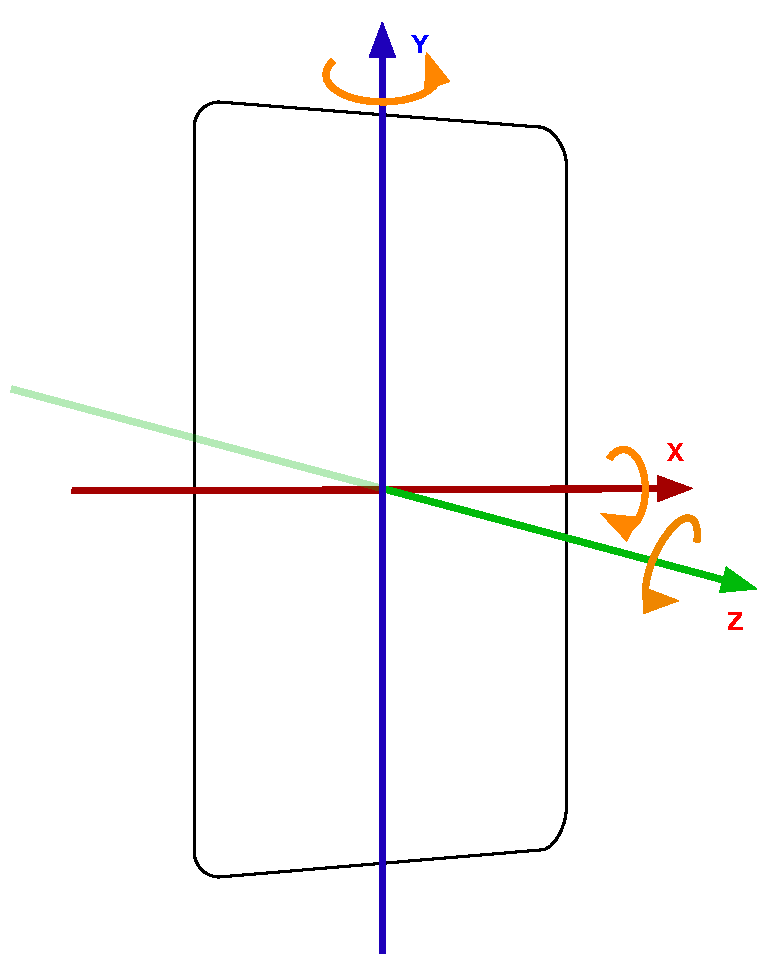
\includegraphics[width=50mm, bb=0 0 373 469]{SmartphoneSensor.pdf}
        \caption{モーションセンサの座標系}
        \label{sensor}
    \end{center}
\end{wrapfigure}

\subsection{加速度センサ}
加速度センサとは,X軸,Y軸,Z軸の基準軸に対して直線運動の加速度をそれぞれ検出し,値として取り出すことの出来るセンサである.
ここでいう加速度とは,端末における単位時間あたりの速度の変化率のことを指し,図\ref{sensor}における直線で示した矢印の方向が正の値,逆が負の値をとる.

\subsection{ジャイロセンサ}
ジャイロセンサとは,X軸,Y軸,Z軸の基準軸に対して回転運動の角速度をそれぞれ検出し,値として取り出すことの出来るセンサである.
ここでいう角速度とは,端末における単位時間あたりの回転角のことを指し,図\ref{sensor}における橙色で示した回転の方向が正の値,逆が負の値をとる.
\end{comment}

% 増幅-ローパス-ずらし
\section{本研究のシステム}
本研究では,兎澤の研究\cite{tozawa}で挙げられていた全体的な認証成功率の低さ,特に手首を中心とするような比較的動きの小さいモーションに対する認証成功率の改善を目標とする.
システムの動作フローを図\ref{flow}に示す.

\begin{wrapfigure}{r}{80mm}
    \begin{center}
        %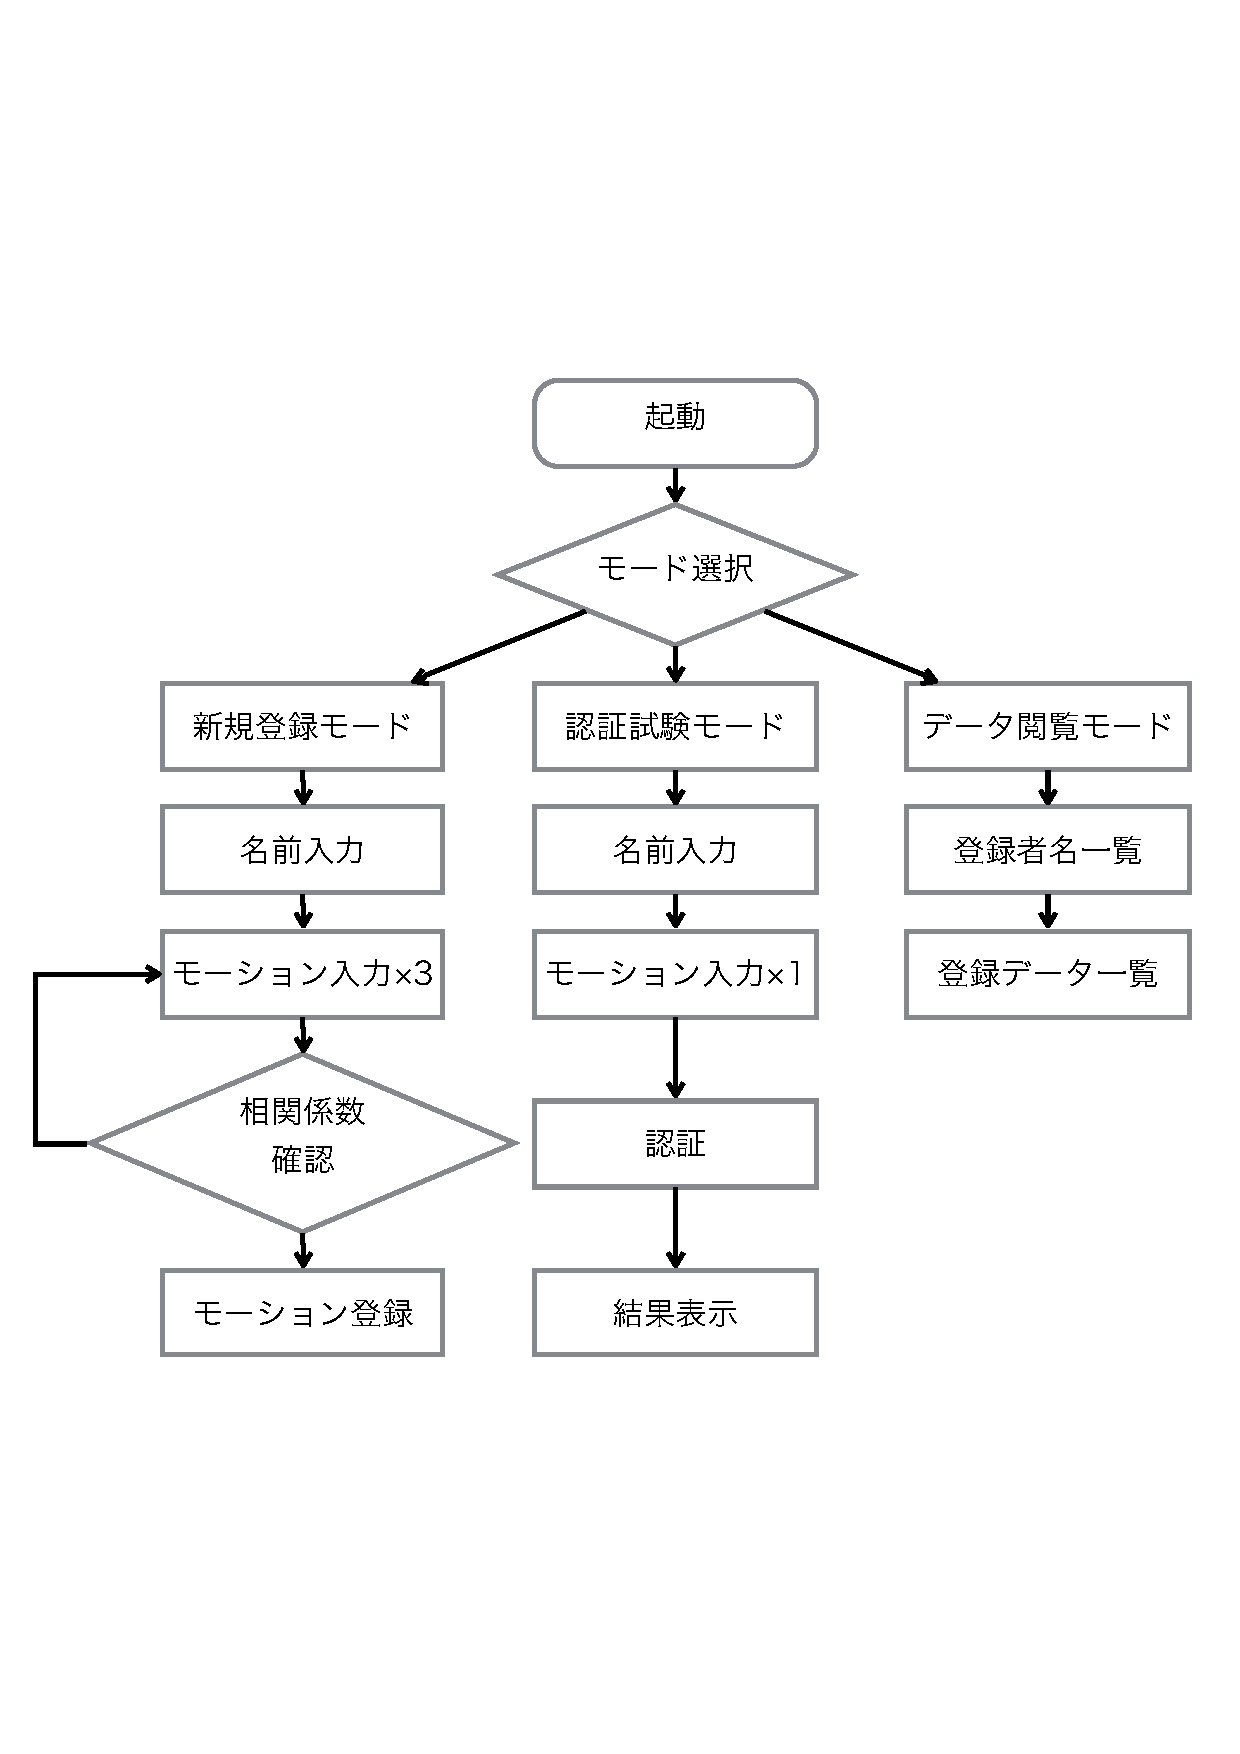
\includegraphics[width=70mm, bb=0 183 594 670]{Flow.pdf}
        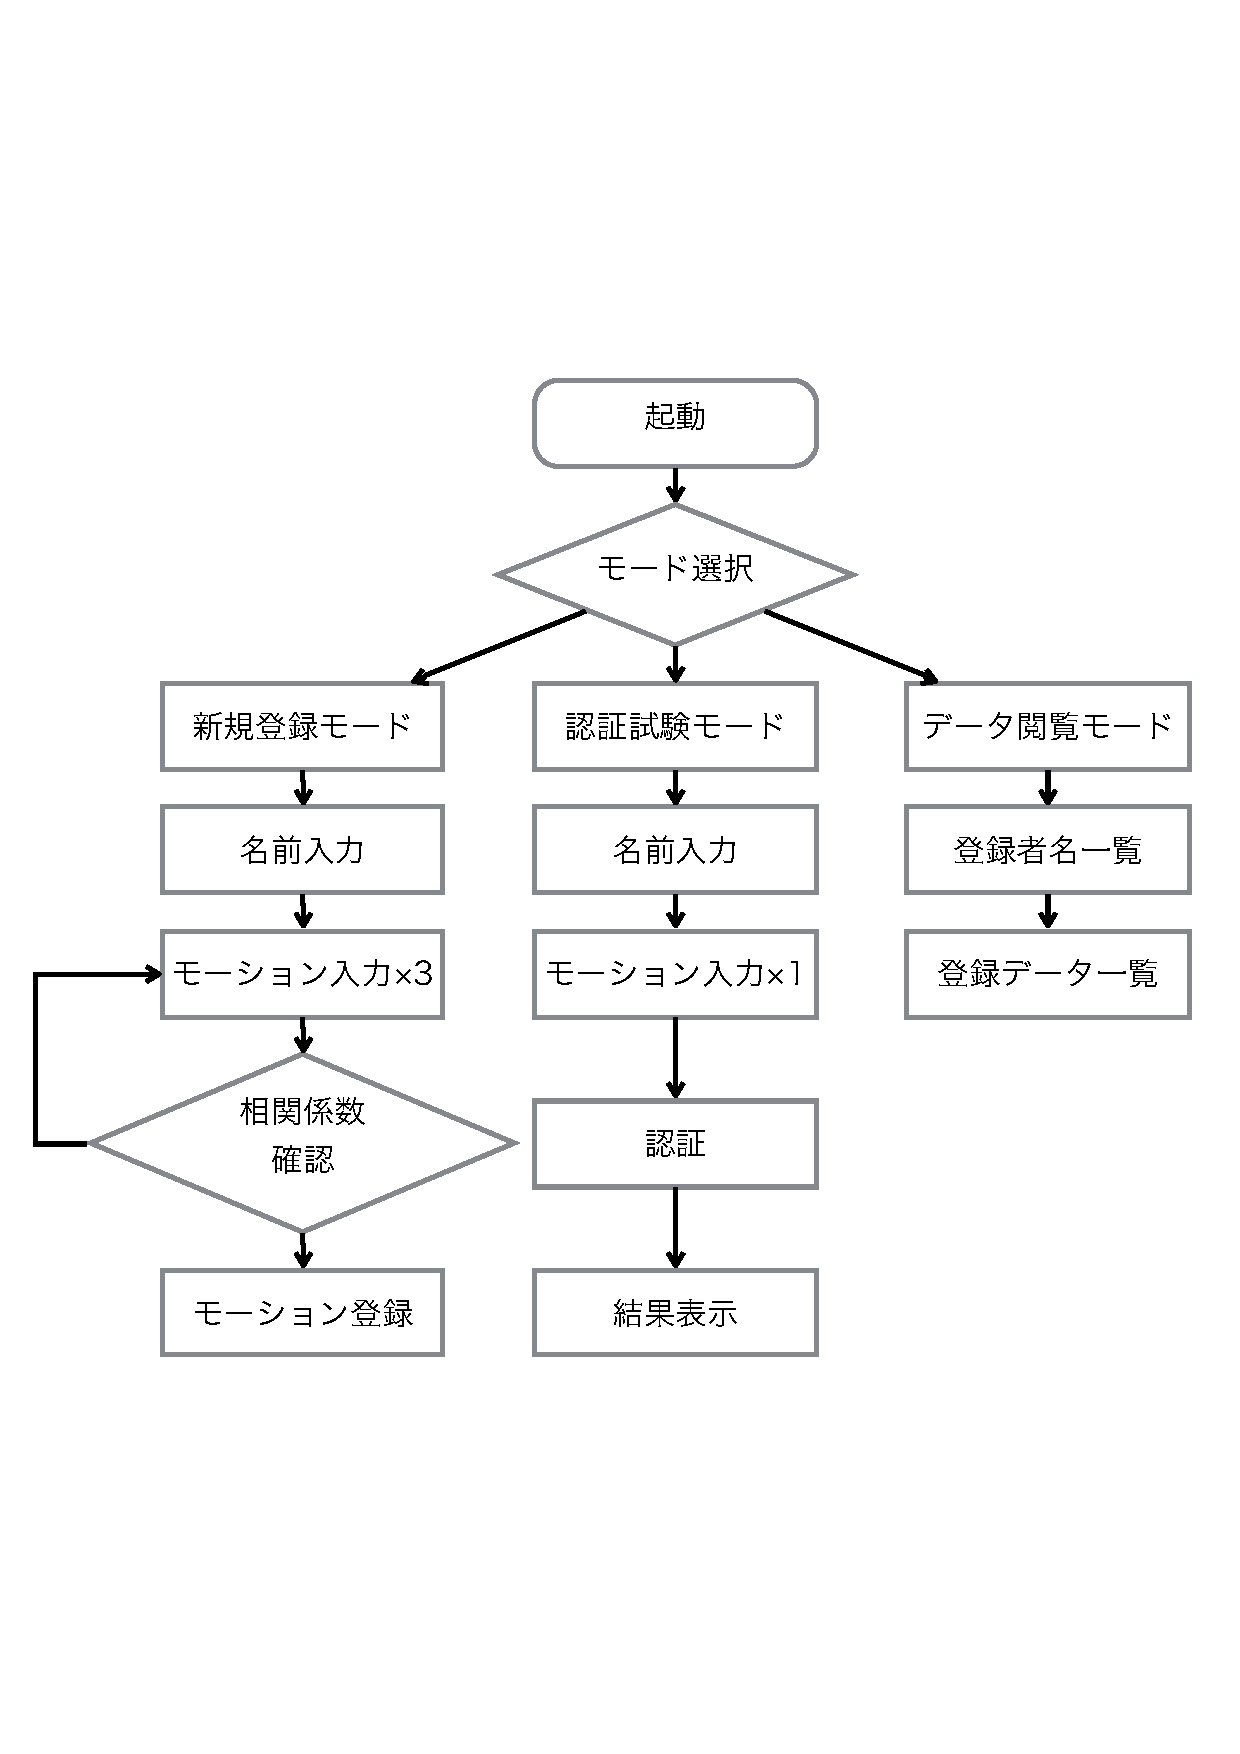
\includegraphics[width=80mm, bb=0 183 590 670]{Flow.pdf}
        \caption{動作フロー図}
        \label{flow}
    \end{center}
\end{wrapfigure}

はじめに,アプリケーション起動後に表示されるモード選択ダイアログより,新規登録モードを選択する.
このモードでは,個人認証を行う際の鍵情報となるモーションデータをユーザ名を指定して登録することができる.
モード選択後,登録したいユーザ名を入力させ,モーションの取得を3回行わせる.
データを取得した後に,その振れ幅を確認する.
あらかじめ設定しておいた増幅器の閾値と増幅量を元に,取得したデータの振れ幅が閾値より小さい場合はモーションの動きが小さいと判断し,データの増幅処理を行う.
次にモーション取得時の手の細かなブレなどから生じうるデータに対する影響を取り除く,フーリエ変換を用いたローパスフィルタ処理を行う.
ローパスフィルタ処理が終われば,取得した回数ごとのデータが同一のモーションのものであるかの確認を行い,確認されればモーション取得時に生じうる時間的なズレを必要に応じて修正する.
時間的なズレを修正する処理が終われば,処理を行った3回分のデータの平均値を算出し,登録する.

これらの処理を行うことで,先行研究で挙げられていた認証成功率の低さや対応できるモーションに限りがあるという問題に対応している.

認証試験モードでは,あらかじめ新規登録モードにおいてモーションデータの登録を行ったユーザ名を指定し,そのデータと新たに1回入力したモーションデータとの相関係数を算出して個人認証を行う.
この際,新規登録モードにおいて登録されたデータに増幅処理がなされていた場合は,新たに入力されたデータに対しても同様の増幅処理を行う.

データ閲覧モードでは,新規登録モードにおいて登録したユーザ名およびモーションデータをリスト形式で閲覧する事ができる.

\section{実験と考察}
\textcolor{red}{冬季休業明けに実験を行う予定です.}
先行研究の課題として挙げられていた,手首を中心とするような比較的小さいモーションに対する認証精度を確認するために,認証の成功率を求める実験を行った.
新規登録モードにおいてあらかじめ登録しておいた以下のモーションそれぞれに対し,認証試験モードにおいて認証を10回ずつ行い,その成功率を求めた.

\begin{itemize}
    \item 円を描くモーション
    \item 三拍子を振るモーション
    \item 四拍子を振るモーション
    \item 無限大記号を描くモーション
    \item 四角形を描くモーション
\end{itemize}

実験結果は,以下の表\ref{result}に示すようになった.

% 実験結果
\begin{table}[htb]
    \begin{center}
        \caption{実験結果}
        \label{result}
        \begin{tabular}{|c|r|} \hline
            モーション & 成功率 \\ \hline \hline
            円を描くモーション & 100\% \\ \hline
            三拍子を振るモーション & 90\% \\ \hline
            四拍子を振るモーション & 90\% \\ \hline
            無限大記号を描くモーション & 100\% \\ \hline
            四角形を描くモーション & 100\% \\ \hline
        \end{tabular}
    \end{center}
\end{table}

今回の実験より,本システムは先行研究に比べて手首を中心とするような動きの小さいモーションに対して高い認証精度を持つことが確認できた.
これにより,先行研究で挙げられていた,手首を中心とするような動きの小さいモーションに対する認証成功率の改善を実現することが出来たと言える.

\section{今後の課題}
本研究により,スマートフォンのモーションセンサを用いた個人認証において生体認証システムの精度を測る指標として挙げられる本人拒否率を下げることが出来た.
しかし,もう一つの指標である他人受入率に関しては検証が不十分である.
具体的には,第三者にモーションの入力を覗き見られ,なりすましによる認証が行われた場合に認証が通ってしまうのかどうかを検証する必要がある.
また,本研究ではモーションの入力時間を3秒間と決めているが,この時間をユーザによって任意に決められる方が,より多彩なモーションを登録できることでユーザにとってシステムがより使いやすくなるという点,また個人認証の要素として端末の動かし方に加えてモーションの時間が加わるため,他人受入率を下げられる可能性があるという点の以上2点が見込まれるため,改善が望ましいと考える.
また,ユーザがモーションを登録したあと,ある程度の期間をおいて個人認証を行った際に,どの程度の割合で認証に成功するかの確認を行う必要がある.

 % 参考文献
\begin{thebibliography}{9}
    \bibitem{tozawa}兎澤星伸,”三軸加速度センサ及び三軸ジャイロセンサを用いた認証アプリケーションの開発”,2012年度卒業研究.
\end{thebibliography}

\end{document}
